%%%%%%%%%%%%%%%%%%%%%%%%%%%%%%%%%%%%%%%%%
% Daily Laboratory Book
% LaTeX Template
%
% This template has been downloaded from:
% http://www.latextemplates.com
%
% Original author:
% Frank Kuster (http://www.ctan.org/tex-archive/macros/latex/contrib/labbook/)
%
% Important note:
% This template requires the labbook.cls file to be in the same directory as the
% .tex file. The labbook.cls file provides the necessary structure to create the
% lab book.
%
% The \lipsum[#] commands throughout this template generate dummy text
% to fill the template out. These commands should all be removed when 
% writing lab book content.
%
% HOW TO USE THIS TEMPLATE 
% Each day in the lab consists of three main things:
%
% 1. LABDAY: The first thing to put is the \labday{} command with a date in 
% curly brackets, this will make a new page and put the date in big letters 
% at the top.
%
% 2. EXPERIMENT: Next you need to specify what experiment(s) you are 
% working on with an \experiment{} command with the experiment shorthand 
% in the curly brackets. The experiment shorthand is defined in the 
% 'DEFINITION OF EXPERIMENTS' section below, this means you can 
% say \experiment{pcr} and the actual text written to the PDF will be what 
% you set the 'pcr' experiment to be. If the experiment is a one off, you can 
% just write it in the bracket without creating a shorthand. Note: if you don't 
% want to have an experiment, just leave this out and it won't be printed.
%
% 3. CONTENT: Following the experiment is the content, i.e. what progress 
% you made on the experiment that day.
%
%%%%%%%%%%%%%%%%%%%%%%%%%%%%%%%%%%%%%%%%%
%idxtotoc,
%----------------------------------------------------------------------------------------
%	PACKAGES AND OTHER DOCUMENT CONFIGURATIONS
%----------------------------------------------------------------------------------------

\documentclass[hyperref,openany, oneside]{labbook} % 'openany' here removes the gap page between days, erase it to restore this gap; 'oneside' can also be added to remove the shift that odd pages have to the right for easier reading

\usepackage[ 
  backref=page,
  pdfpagelabels=true,
  plainpages=false,
  colorlinks=true,
  bookmarks=true,
  pdfview=FitB]{hyperref} % Required for the hyperlinks within the PDF
  
\usepackage{booktabs} % Required for the top and bottom rules in the table
\usepackage{float} % Required for specifying the exact location of a figure or table
\usepackage{graphicx} % Required for including images
\usepackage{lipsum} % Used for inserting dummy 'Lorem ipsum' text into the template

\usepackage{listings}
\usepackage{color}
\usepackage[margin=0.5in]{geometry}


\graphicspath{{../Figures/}}

\definecolor{green}{rgb}{0,0.5,0}
\definecolor{gray}{rgb}{0.5,0.5,0.5}
\definecolor{mauve}{rgb}{0.58,0,0.82}
\definecolor{red}{rgb}{0.8,0,0}

\lstset{frame=tb,
  language=Python,
  aboveskip=3mm,
  belowskip=3mm,
  showstringspaces=false,
  columns=flexible,
  basicstyle={\small\ttfamily},
  numbers=none,
  numberstyle=\tiny\color{gray},
  keywordstyle=\color{mauve},
  commentstyle=\color{red},
  stringstyle=\color{green},
  breaklines=true,
  breakatwhitespace=true,
  tabsize=3
}

\newcommand{\HRule}{\rule{\linewidth}{0.5mm}} % Command to make the lines in the title page
\setlength\parindent{0pt} % Removes all indentation from paragraphs

%----------------------------------------------------------------------------------------
%	DEFINITION OF EXPERIMENTS
%----------------------------------------------------------------------------------------

\newexperiment{DNA}{Very Abbreviated History of DNA}
\newexperiment{Ancestry}{Ancestry: Origin of Your DNA}
\newexperiment{Gattac}{Genes Maketh the Man?}
\newexperiment{Law}{You as Defined by Merriam-Webster}
%\newexperiment{shorthand}{Description of the experiment}

%---------------------------------------------------------------------------------------

\begin{document}

%----------------------------------------------------------------------------------------
%	TITLE PAGE
%----------------------------------------------------------------------------------------

\frontmatter % Use Roman numerals for page numbers
\title{
\begin{center}
\HRule \\[0.4cm]
{\Huge \bfseries Kollel Genetics Talk \\[0.5cm] \Large} % Degree
\HRule \\[1.5cm]
\end{center}
}
\author{\Huge Cody Glickman \\ \\ \LARGE cody.glickman@ucdenver.edu \\[2cm]} % Your name and email address
\date{October 2018} % Beginning date
% \maketitle

%\tableofcontents

\mainmatter % Use Arabic numerals for page numbers

%----------------------------------------------------------------------------------------
%	LAB BOOK CONTENTS
%----------------------------------------------------------------------------------------
\labday{Kollel Genetics}

\experiment{DNA}
\vspace{-0.3cm}
1952: Hershey-Chase experiment define deoxyribonucleic acid (DNA) as genetic material \\
1953: DNA double helix structure described by Rosalind Franklin, James Watson, and Francis Crick
\vspace{-0.5cm}
\begin{center}
	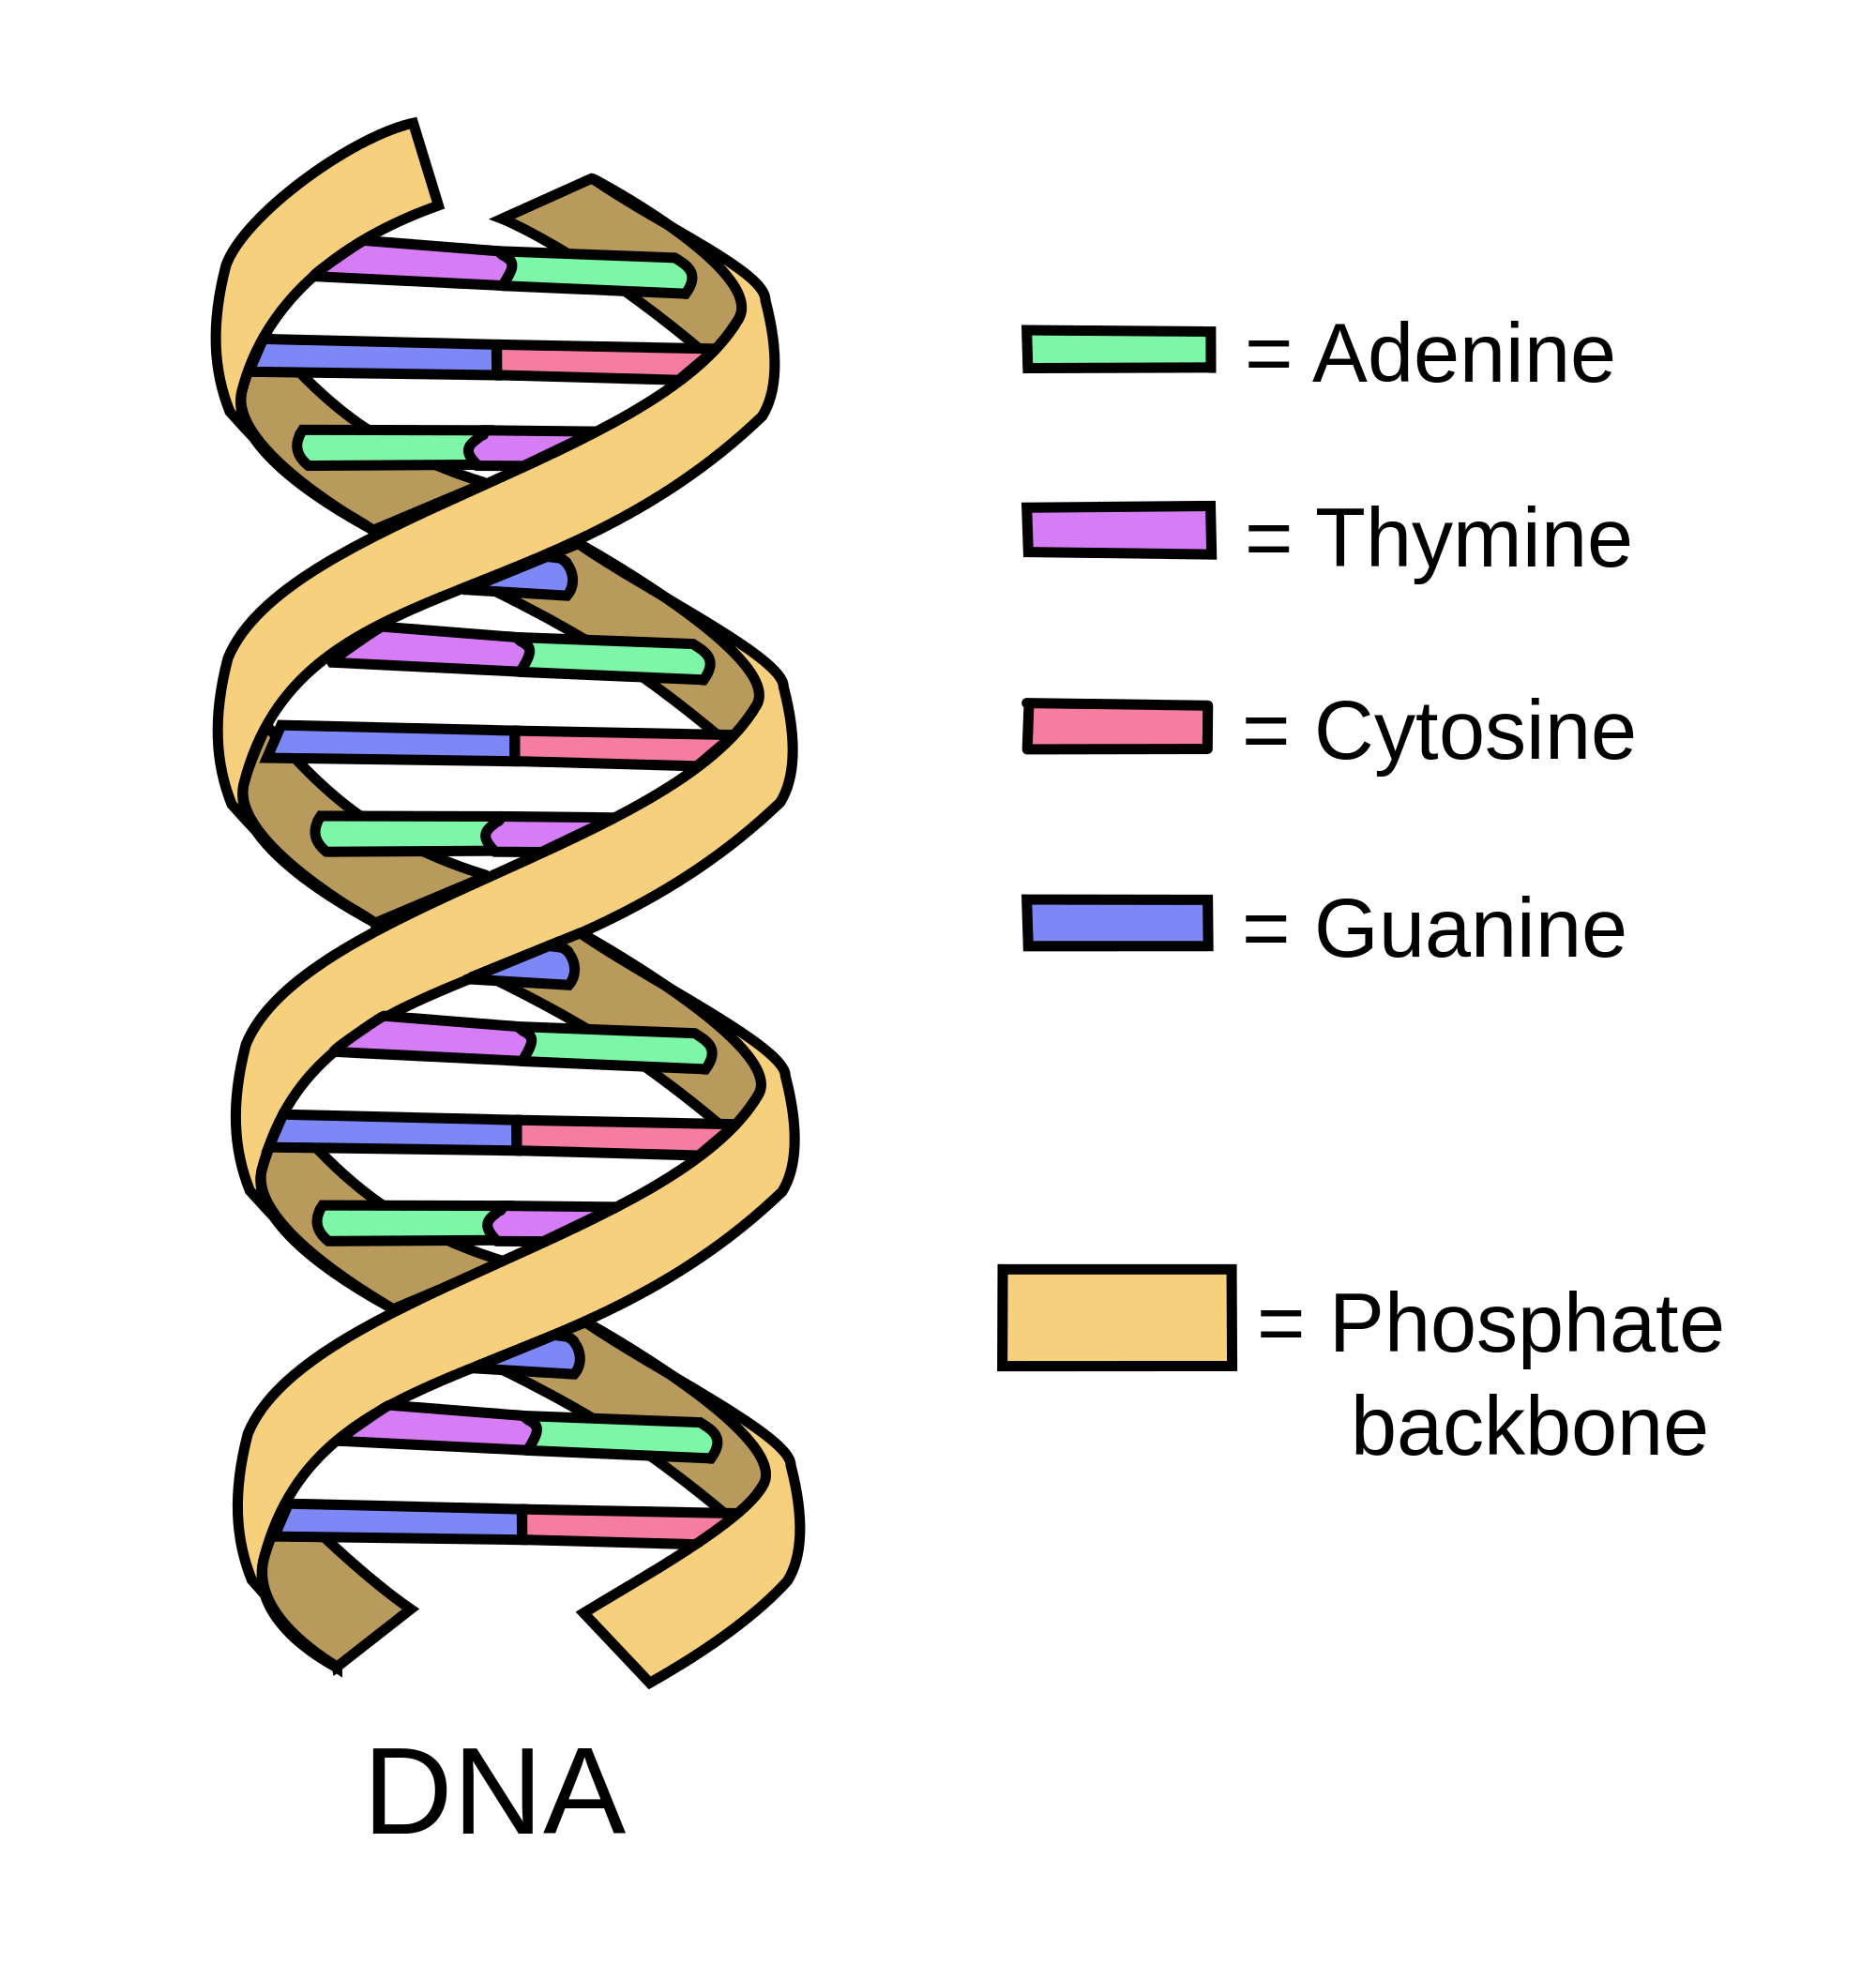
\includegraphics[height=4cm, width=4.5cm]{dnastructure.png}{\textbf{like baseball - 4 bases}}
\end{center}
\vspace{-0.2cm}
1977: Sanger sequencing is developed, the foundation of current sequencing methods 
\\
1990 - 2003: Human Genome Project estimates about 25K genes 
\\
2009: Third generation long-read sequencing is introduced



\vspace{-0.4cm}

\experiment{Ancestry}
\vspace{-0.3cm}
\underline{Your cells contain \textbf{3} categories of DNA} \\
1. Somatic: Chromosomal DNA \\
2. Sex Chromosomes: X \& Y Chromosomes \\
3. Mitochondrial DNA: Only about 16K base pairs encoding 37 genes \\


There are \textbf{3} types of ancestry testing: Mitochondrial (Material), Y-Chromosome (Paternal), Somatic (Regional)
\begin{center}
	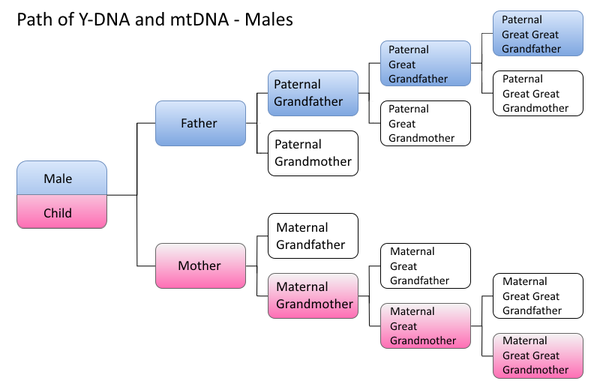
\includegraphics[height=5cm, width=8cm]{Paths.png}
\end{center}

Short Tandem Repeats (STRs) are small, 2-7 base pairs, repeated units in DNA. STRs are typically use for recent genealogical information (i.e. determining extended familial relationships or identifying a suspect in a crime). For example, Cohan Modal Haplotype (CMH) is a pattern of 12 Y-STRs present primarily in the Kohanim.
\vspace{-0.3cm}
\begin{center}
	\begin{tiny}
		Hammer, Michael F., et al. "Extended Y chromosome haplotypes resolve multiple and unique lineages of the Jewish priesthood." Human genetics. 2009
	\end{tiny}\\
	
\includegraphics[height=0.5cm, width=5cm]{str-example.png}
\end{center}

STRs are not used in Somatic testing commonly associated with DNA ancestry. Single Nucleotide Polymorphisms (SNPs) are point mutations in DNA strings compared to a genome reference. There are \textbf{a lot} of point mutations between groups. 

\begin{center}
	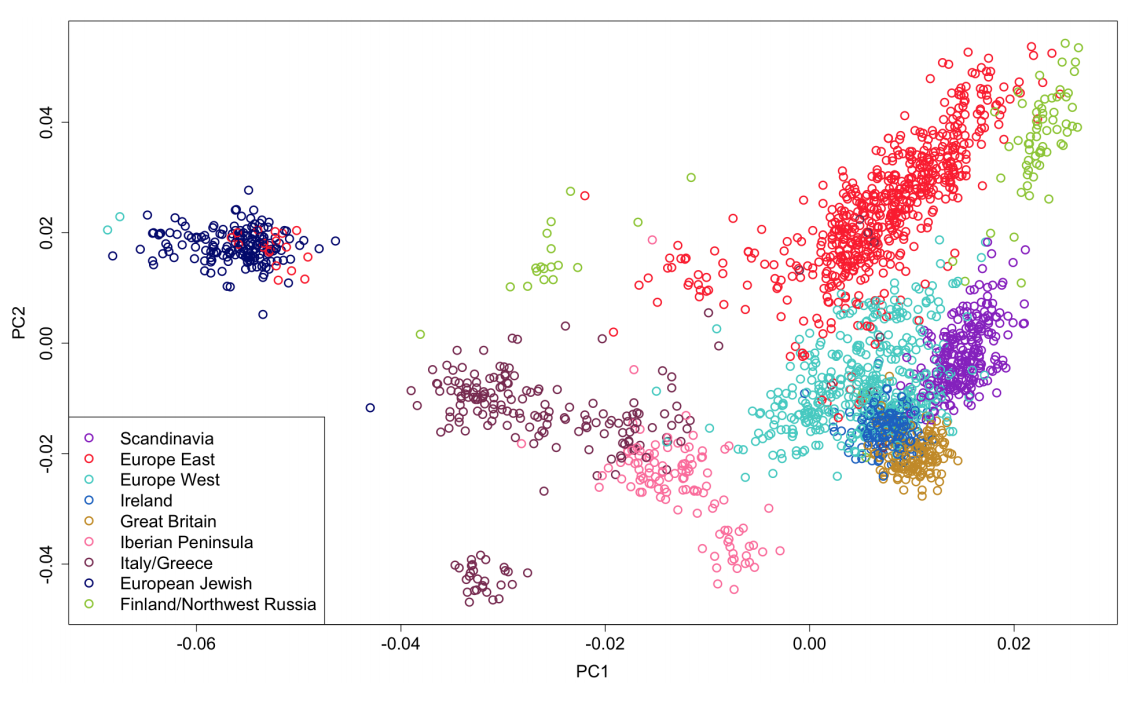
\includegraphics[height=5cm, width=5.5cm]{kollel_1.png}\\
	\begin{tiny}
		Ball, C., et al. AncestryDNA. Ethnicity Estimate White Paper. 2013.
	\end{tiny}
\end{center}

SNP testing is able to identify \textbf{3} branches common to Jewish lineages: Ashkinazi (Eastern Europe), Sephardic (North Africa), and Mizrahi (Middle East). 

\begin{center}
	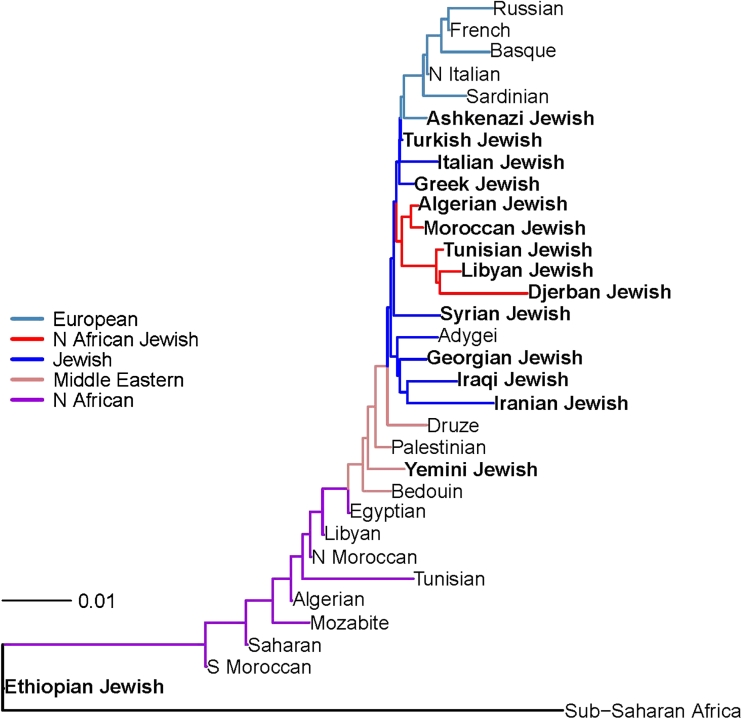
\includegraphics[height=5cm, width=5.5cm]{treejew.jpg}\\
	\begin{tiny}
		Ostrer, Harry, and Karl Skorecki. "The population genetics of the Jewish people." Human genetics 132.2 (2013): 119-127.
	\end{tiny}
\end{center}

\vspace{-0.3cm}
\experiment{Gattac}
\vspace{-0.2cm}
Incomplete penetrance is term that defines an individual that carries a genetic mutation, however does not express the trait. 

\begin{center}
	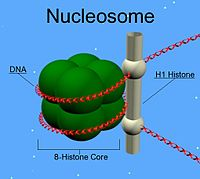
\includegraphics[height=3cm, width=3.5cm]{Nucleosome.jpg}
\end{center}

Epigenetics affects expression of traits generation downstream of environmental stimulus. 
\begin{center}
	The answer to the question of nature vs. nurture is both.
\end{center}

\vspace{-0.3cm}
\experiment{Law}
\vspace{-0.2cm}
You are genetically unique and thus \textbf{Genetically Identifiable}. The Genetic Information Nondiscrimination Act (GINA) passed in 2008 to protect from genetic discrimination in health insurance and employment. Sequencing information provided by a close relative can be used to partially identify you. DNA is very stable and can be stored for long periods of time (long after your lifespan).

\textbf{Open Questions:}\\
Does your genetic information define your identity? \\ 
To what extent are your genetics representative of your physical traits? \\
Who should be allowed to see your genetic information?


\end{document}